\documentclass[10pt]{article}
\usepackage[T1]{fontenc}
\usepackage{ae,aecompl}
\usepackage[utf8x]{inputenc}
\usepackage[cm]{fullpage}
%\usepackage{mdwlist}
%\usepackage[small]{caption}
\usepackage[numbers,sort&compress,square]{natbib}
\usepackage{ctable}
%\makeatletter
%\renewcommand\bibsection%
%{
%  \section*{\refname
%    \@mkboth{\MakeUppercase{\refname}}{\MakeUppercase{\refname}}}
%}
%\makeatother

\usepackage{times}
\usepackage{amsfonts}
\usepackage{amsmath}
\usepackage{amssymb}
\usepackage{amsthm}
\usepackage{dsfont}
\usepackage{mathtools}
\usepackage{graphicx}
\usepackage{subfig}
\usepackage{multirow}
\usepackage{bigstrut}
\usepackage{url}
\usepackage[ruled,linesnumbered]{algorithm2e}
\usepackage{mathptmx}      % use Times fonts in math if available on your TeX system
\DeclareMathAlphabet{\mathcal}{OMS}{cmsy}{m}{n} % Use standard fonts for calligraphic

\newtheorem{corollary}{Corollary}
\newtheorem{conj}{Conjecture}
\newtheorem{lemma}{Lemma}
\newtheorem{claim}{Claim}
\newtheorem{theorem}{Theorem}

\theoremstyle{definition}
\newtheorem{definition}{Definition}

\def\XXX{{\bf XXX}}
\def\MR{{\bf MR}}
\def\EK{{\bf EK}}

\def\prob{\pi}
\def\range{\mathcal{R}}
\def\VC{\mathsf{VC}}

\title{Approximating Betweenness Centrality through Sampling with the
VC-Dimension}
\author{ }
\begin{document}
\maketitle

\begin{abstract}
  We present an efficient randomized algorithm for approximating the {\sl
  betweenness centrality} of all nodes in a network within strict probabilistic
  guarantees.  Betweenness centrality is a fundamental measure in social network
  analysis, quantifying the importance or influence of individual nodes in a
  network in terms of the number of shortest paths (between all pairs of nodes
  in the network) that pass through that node. The fastest known algorithm to
  compute the exact betweenness of all vertices in a graph $G=(V,E)$ in
  $O(|V|\cdot|E|)$ steps in the unweighted case and in
  $O(|V|\cdot|E|+|V|^2\log|V|)$ steps in weighted graphs. Exact computation in
  large networks with millions of vertices and hundred of millions of edges is
  therefore prohibitively expensive and fast approximation algorithms are
  required in these cases. Our novel algorithm computes an
  $(\epsilon,\delta)$-approximation of the vector of betweenness centrality of
  all the nodes in the graph. Our algorithm is significantly faster than any
  other algorithm with similar approximation guarantees. We achieve this speed
  up through a novel application of the VC-dimension method for optimizing the
  sampling component of the algorithm. Extensive experimental evaluation on real
  and artificial networks demonstrate the practicality of our method and its
  speed up compared to exact and other known approximated solutions for this
  problem.
\end{abstract}
  

\section{Introduction}\label{sec:intro}
\XXX TBD

\paragraph{Our contributions} 
We present two randomized algorithms to approximate the betweenness centrality
(and some of its variants) of vertices of a graph. The first algorithm
guarantees that the estimated betweenness values for all vertices are within an
\emph{additive} factor $\varepsilon$ from the real values, with probability at
least $1-\delta$. The second algorithm focuses on the top-$K$ vertices with
highest betweenness and returns a set of vertices which includes the top-$K$,
while ensuring that the estimated betweenness for all returned vertices is
within a \emph{multiplicative} factor $\varepsilon$ from the real value, with
probability at least $1-\delta$. This is the first algorithm to reach such a
high-quality approximation for the set of top-$K$ vertices. The algorithms are
based on random sampling of shortest paths. The analysis to derive the
sufficient sample size uses notions and tools from VC-Dimension theory. This
results in a much smaller sample size than that used by other algorithms
guaranteeing the same approximation. Moreover, the amount of work performed by
our algorithms per sample is also less than what was done in previous works.
We extensively evaluated our methods on real graphs and compared their
performances to the exact algorithm for betweenness
centrality~\citep{Brandes01} and to other sampling-based approximation
algorithms~\citep{JacobKLPT05,BrandesP07}.



\section{Related work}\label{sec:prevwork}
Over the years, a number of centrality measures have been defined. In this work
we are only concerned with betweenness centrality and some of its variants. We
refer the reader interested in other measure to the book by~\citet{Newman10} and
references therein.

Betweenness centrality was introduced in the sociology
literature~\citep{Anthonisse71,Freeman77}. 

Variants~\citep{Brandes08,DolevEP10,KourtellisASIT12,PfefferC12}

The need of fast algorithms to compute
the betweenness of vertices in a graph arose as large online social networks
developed. \citet{Brandes01} presents the first efficient algorithm for the
task, running in time $O(|V|\cdot|E|)$ on unweighted graphs and
$O(|V|\cdot|E|+|V|^2\log|V|)$ on weighted ones. The algorithm computes, for each
vertex $v$, the shortest path to every other vertex and then traverses these paths
backwards to efficiently compute the contribution of the shortest paths from $v$
to the betweenness of other vertices. For very large networks, the cost of this
algorithm would still be prohibitive in practice, so many approximation
algorithms were
developed~\citep{JacobKLPT05,BrandesP07,BaderKMM07,GeisbergerSS08,MaiyaBW10,LimMRT11}.
The use of random sampling was one of the more natural approaches to speed up
the computation of betweenness. Inspired by the work of~\citet{EppsteinW04},
\citet{JacobKLPT05,BrandesP07} present an algorithm that samples vertices at
random and compute the contribution of the sampled vertices to the betweenness
of every vertex. The number of samples needed to guarantee that, with
probability at least $1-\delta$, the estimate for each node is within
$\binom{|V|}{2}\varepsilon$ from the real value, for some $\varepsilon\in(0,1)$,
is $O(\log(n/\delta)/\varepsilon^2)$. The analysis uses Hoffeding bounds and the
union bound. The algorithm mimics the exact one, with the difference
that, instead of computing the contribution of all vertices to the betweenness
of the others, only it only consider the contribution of the sampled vertices.
\citet{GeisbergerSS08} noticed that this can lead to an overestimation of the
betweenness of vertices that are close to the sampled ones and introduced
different unbiased estimators that are experimentally shown to have smaller
variance and do not occur in this overshooting. Our algorithm is different
because each sample in our case is a single random shortest path between two
randomly chosen nodes. This leads to a much smaller sample size and less work
done for each sample, resulting in a much faster way to compute approximations
of the betweenness with the same probabilistic guarantees. We delve more in the
comparisons with these algorithm in Sect.~\ref{sec:discussion}
and~\ref{sec:exper}.
A number of works explored the use of adaptive sampling, in contrast with the
previous algorithms (and ours) which use a fixed sample size. \citet{BaderKMM07}
present an adaptive sampling algorithm which computes good estimations for the
betweenness of high-centrality vertices, by keeping track of the partial
contribution of each sampled vertex, obtained by performing a single-source
shortest paths computation to all other vertices. \citet{MaiyaBW10} use concepts
from expander graphs to select a connected sample of vertices which includes the
highest centrality ones and such that the betweenness computed on the induced
sample subgraph is close to the real one. They achieve these by repeatedly
including in the sample the vertex in the neighborhood of the sample which
maximizes the number of connections with vertices not already in the sample.
Modified versions of this algorithm and an extensive experimental evaluation
appeared in~\citep{LimMRTB11}. The algorithm does not offer any guarantee on the
quality of the approximations. Compared to these adaptive sampling approaches,
our method ensures that the betweenness of all vertices is well approximated
with a fixed, predetermined amount of samples.

Other approximations~\citep{GkorouPE10,PrountzosP13,SaryuceSKC13}

VC-Dimension on graphs~\citep{AnthonyBC95,KranakisKRUW97,MubayiZ07,YcartR07}
(mostly only~\citep{KranakisKRUW97}

VC-Dimension and Shortest paths~\citep{AbrahamDFGW11}


\section{Preliminaries}\label{sec:prelims}
In this section we introduce the definitions and lemmas that we will use to
develop and analyze our results throughout the paper.

\subsection{Graphs and betweenness centrality}\label{sec:graphprelims}
Let $G=(V,E)$ be a graph, where $E\subseteq V\times V$, with $n=|V|$ vertices
and $m=|E|$ edges. The graph $G$ can be directed or undirected. We assume that
there are no self-loops from one vertex to itself and no multiple edges between
a pair of vertices. Each edge $e\in E$ has a non-negative weight
$\mathsf{w}(e)$. Given a pair of distinct vertices $(u,v)\in V\times V$,
$u\neq v$, a \emph{path $p_{uv}\subseteq V$ from $u$ to $v$} is an ordered sequence of
vertices $p_{uv}=(w_1,\dotsc,w_{|p_{uv}|})$ such that $w_1=u$, $w_{|p_{uv}|}=v$ and
for each $1\le i < |p_{uv}|$, $(w_i,w_{i+1})\in E$. The vertices $u$ and $v$ are
called the \emph{end points} of $p_{uv}$ and the vertices in
$\mathsf{Int}(p_{uv})=p_{uv}\setminus\{u,v\}$ are the \emph{internal vertices of
$p_{uv}$}. The \emph{weight}
$\mathsf{w}(p_{uv})$ of a path $p_{uv}=(u=w_1,w_2,\cdots,w_{p_{|uv|}}=v)$ from
$u$ to $v$ is the sum of the weights of the edges composing the path:
$\mathsf{w}(p_{uv})=\sum_{i=1}^{|p_{uv}|-1}\mathsf{w}((w_i,w_{i+1}))$. We denote with
$|p_{uv}|$ the number of vertices composing the path and call this the
\emph{size of the path $p_{uv}$}. Note that if the weights are not all unitary,
it is not necessarily true that $\mathsf{w}(p_{uv})=|p_{uv}|-1$. A special and
degenerate path is the \emph{empty path} $p_{\emptyset}=\emptyset$, which by
definition has weight $\mathsf{w}(p_\emptyset)=\infty$, no end points, and
$\mathsf{Int}(p_\emptyset)=\emptyset$.

Given two distinct vertices $(u,v)\in V\times V$, the \emph{shortest path distance}
$d_{uv}$ between $u$ and $v$ is the weight of a path with minimum weight 
between $u$ and $v$ among all paths between $u$ and $v$. If there is no path
between $u$ and $v$, $d_{uv}=\infty$. We call a path between $u$ and $v$ with
weight $d_{uv}$ a \emph{shortest path between $u$ and $v$}. There can be
multiple shortest paths between $u$ and $v$ and we denote the set of these paths
as $\mathcal{S}_{uv}$ and the number of these paths as
$\sigma_{uv}=|\mathcal{S}_{uv}|$. If there is no path between $u$ and $v$, then
$\mathcal{S}_{uv}=\{p_\emptyset\}$\footnote{Note that even if
$p_\emptyset=\emptyset$, the set $\{p_\emptyset\}$ is not empty. It contains
one element.}.
%By definition, $\mathcal{S}_{vv}=\emptyset$.
We denote with $\mathbb{S}_G$ the union of all the $\mathcal{S}_{uv}$'s, for all
pairs $(u,v)\in V\times V$ of distinct nodes $u\neq v$: 
\[ \mathbb{S}_G=\bigcup_{\substack{(u,v)\in V\times V \\ u\neq v}}\mathcal{S}_{uv}\enspace.\]

We now define a characteristic quantity of a graph that we will use throughout
the paper.
\begin{definition}\label{def:vertexdiam}
  Given a graph $G=(V,E)$, the \emph{vertex-diameter $\VD(G)$ of $G$} is the
  size of the shortest path in $G$ with maximum size:
  \[
  \VD(G) = \max\left\{|p| ~:~ p\in \mathbb{S}_G\right\}\enspace.\]
\end{definition}
The vertex-diameter is the maximum number of vertices among all shortest paths
in $G$. If all the edge weights are unitary, then $\VD(G)$ is equal to
$\mathsf{diam}(G)+1$, where $\mathsf{diam}(G)$ is the number of edges composing
the longest shortest path in $G$. 
%\XXX Shall we make an example with a figure?

Given a vertex $v$, let $\mathcal{T}_v\subseteq\mathbb{S}_G$ be the set of all
shortest paths that $v$ is \emph{internal} to:
\[
\mathcal{T}_v=\{p\in\mathbb{S}_G ~:~ v\in\mathsf{Int}(p)\}\enspace.
\]
In this work we are interested in the \emph{betweenness centrality} of the
vertices of a graph.

%\begin{definition}[\citep{Anthonisse71,Freeman77}]\label{def:betwenness}
\begin{definition}\label{def:betwenness}
  \citep{Anthonisse71,Freeman77} Given a graph $G=(V,E)$, the \emph{betweenness
  centrality of a vertex $v\in V$} is defined as\footnote{We use the normalized
  version of betweenness as we believe it to be more suitable for presenting
  approximation results.}
  \[
  \betw(v)=\frac{1}{n(n-1)}\sum_{p_{uw}\in\mathbb{S}_G}\frac{\mathds{1}_{\mathcal{T}_v}(p)}{\sigma_{uv}}%=\frac{1}{n(n-1)}\sum_{p_{uw}\in\mathcal{T}_v}\frac{1}{|\mathcal{S}_{uw}|}
  \enspace.
  \]
\end{definition} 

It is easy to see that $\betw(v)\in[0,1]$. \citet{Brandes01} presented an
algorithm to compute the betweenness centrality for all $v\in V$ in time
$O(nm)$ for unweighted graphs and $O(nm + n^2 \log n)$ for weighted graphs. 

\ifproof
\else
A ``local'' variant of betweenness, called \emph{$k$-bounded-distance
betweenness}\footnote{Bounded-distance betweenness is also known as
$k$-betweenness. We prefer the former denomination to avoid confusion with
$k$-path betweenness.} only considers
the contribution of shortest paths of size up to $k+1$~\citep{BorgattiE06,Brandes08}.
For $k>1$ and any pair of distinct vertices $u,v\in V$, $u\neq V$, let
$\mathcal{S}^{(k)}_{uv}\subseteq\mathcal{S}_{uv}$ be the set of shortest paths
from $u$ to $v$ of size at most $k+1$, with
$\sigma^{(k)}_{uv}=|\mathcal{S}^{(k)}_{uv}|$, and let $\mathbb{S}^{(k)}_G$ be the
union of all the $\mathcal{S}^{(k)}_{uv}$. Let
$\mathcal{T}^{(k)}_v\subseteq\mathcal{T}_v$ be the set of all shortest paths
\emph{of size up to $k$} that $v$ is internal to, for each $v\in V$.

%\begin{definition}[\citep{BorgattiE06,Brandes08}]\label{def:kboundbetweenness}
\begin{definition}\label{def:kboundbetweenness}
  \citep{BorgattiE06,Brandes08} Given a graph $G=(V,E)$ and an integer $k>1$,
  the \emph{$k$-bounded-distance betweenness centrality of a vertex $v\in V$} is
  defined as
  \[
  %\betw(v)=\sum_{(u,w)\in V\times
  %V}\sum_{p\in\mathcal{S}_{uw}}\frac{\mathds{1}_{\mathcal{T}_v}(p)}{|\mathcal{S}_{uw}|}\enspace.
  %\betw(v)=\sum_{p_{uw}\in\mathbb{S}_G}\frac{\mathds{1}_{\mathcal{T}_v}(p)}{|\mathcal{S}_{uw}|}\enspace.
  \kboundbetw^{(k)}(v)=\frac{1}{n(n-1)}\sum_{p_{uw}\in\mathbb{S}^{(k)}_G}\frac{\mathds{1}_{\mathcal{T}^{(k)}_v}(p)}{\sigma^{(k)}_{uw}}
  %=\frac{1}{n(n-1)}\sum_{p_{uw}\in\mathcal{T}^{(k)}_v}\frac{1}{\left|\mathcal{S}^{(k)}_{uw}\right|}
  \enspace.
  \]
\end{definition}
\fi

\subsection{Vapnik-Chervonenkis dimension}\label{sec:prelvcdim}
The Vapnik-Chernovenkis (VC) dimension of a class of subsets defined
on a set of points is a measure of the complexity or expressiveness of such
class~\citep{VapnikC71}. Given a probability distribution on the set of points,
a finite bound on the VC-dimension of the class of subsets implies a bound on
the number of random samples required to approximate the probability of each
subset in the class with its empirical average. We outline here some basic
definitions and results and refer the reader to the book by~\citet{MohriRT12}
for an in-depth presentation.
%works of~\citet[Sect.~14.4]{AlonS08} and
%\citet[Sect.~3]{BoucheronBL05} for an introduction of VC-dimension and a survey
%of recent developments. \XXX Cite book Foundations of ML instead.
%~\citet[Sect.~12.4]{DevroyeGL96},
%\citet[Sect.~3]{BoucheronBL05}, \citet[Sect.~14.4]{AlonS08}, and
%\citet{Vapnik99} for more details on VC-dimension.

Let $D$ be a domain and $\range$ be a collection of subsets from $D$. We call
$\range$ a \emph{range set on $D$}.
Given $B\subseteq D$, the \emph{projection of $\range$ on $B$} is the set 
$P_\range(B)=\{ B\cap A ~:~ A\in\range\}$. We say that the set $B$ is
\emph{shattered} by $\range$ if $P_\range(B)=2^B$.

\begin{definition}\label{def:vcdim}
  The \emph{Vapnik-Chervonenkis (VC) dimension of $\range$}, denoted as
  $\VC(\range)$, is the cardinality of the largest subset of $D$ that is
  shattered by $\range$.
\end{definition}

\ifproof
Note that a range space $(X,R)$ with an arbitrary large set of points $X$ and
an arbitrary large family of ranges $R$ can have a bounded VC-dimension. A simple
example is the family of intervals in $[0,1]$ (i.e. $X$ is all the points in
$[0,1]$ and $R$ all the intervals $[a,b]$, such that $0\leq a\leq b\leq 1$). Let
$A=\{x,y,z\}$ be the set of three points $0<x<y<z<1$. No interval in $R$ can
define the subset $\{x,z\}$ so the VC-dimension of this range space is less than
3~\citep[Lemma 10.3.1]{Matousek02}. Another example is shown in
Fig.~\ref{fig:rectangles}.
\begin{figure}[ht]
  \centering
  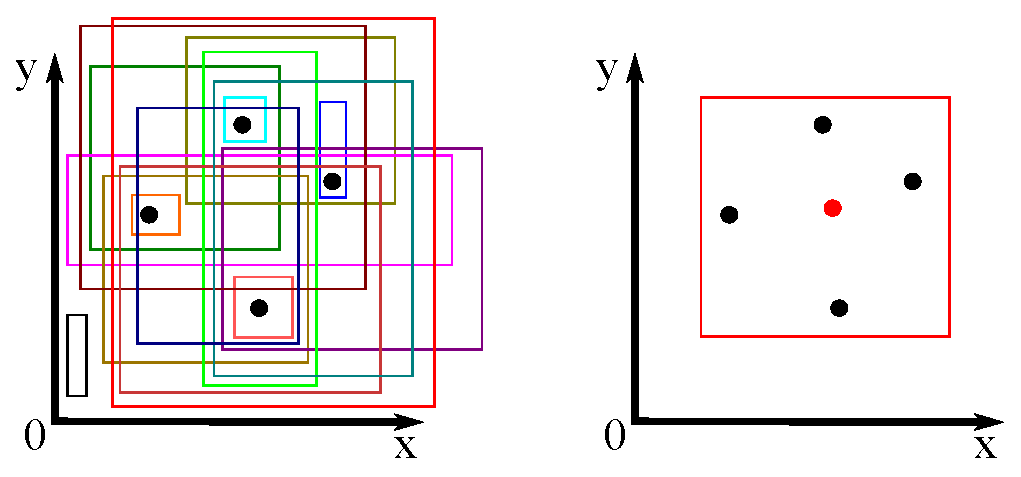
\includegraphics[width=.7\textwidth,keepaspectratio]{figures/rectangles}
  \caption{Example of range space and VC-dimension. The space of points is the
  plane $\mathbb{R}^2$ and the set of ranges is the set of all
  \emph{axis-aligned rectangles}. The figure on the left shows graphically that
  it is possible to shatter a set of four points using 16 rectangles. On the
  right instead, one can see that it is impossible to shatter five points, as,
  for any choice of the five points, there will always be one (the red point in
  the figure) that is internal to the convex hull of the other four, so it would
  be impossible to find an axis-aligned rectangle containing the four points
  but not the internal one. Hence $\VC((X,R))=4$.}
  \label{fig:rectangles}
\end{figure}
\fi

The main application of VC-dimension in statistics and learning
theory is in computing the number of samples needed to approximate the
probabilities of the ranges using their empirical averages as
unbiased estimators. Formally, let $X_1^k=(X_1,\dotsc,X_k)$ be a collection of
independent identically distributed random variables taking values in $D$,
sampled according to some distribution $\phi$ defined on the elements of $D$.
For a set $A\subseteq D$, let $\phi(A)$ be the probability that a sample from
$\phi$ belongs to the set $A$, and let the \emph{empirical average} of $\phi(A)$
on $X_1^k$ be 
\[
\phi_{X_1^k}(A)=\frac{1}{k}\sum_{j=1}^k\mathds{1}_A(X_j)\enspace.%, 
\]
%where $\mathds{1}_A$ is the indicator function for the set $A$. 
The empirical average of $\phi(A)$ can be used as an \emph{unbiased} estimator
for $\phi(A)$.

\begin{definition}\label{def:eapprox}
  Let $\range$ be a range set on %a domain
  $D$ and $\phi$ be a probability distribution on $D$. For $\varepsilon\in(0,1)$,
  an \emph{$\varepsilon$-approximation to $(\range,\phi)$} is a bag $S$ of
  elements of $D$ such that 
  \[
  \sup_{A\in\range}|\phi(A)-\phi_S(A)|\le\varepsilon\enspace.\]
\end{definition}

When an upper bound to the VC-dimension of $\range$ is available, it is possible
to build an $\varepsilon$-approximation by sampling points of
the domain according to the distribution $\phi$.

\begin{theorem}[Thm.~2.12~\citep{HarPS11} (see also~\citep{LiLS01})]\label{thm:eapprox}
  Let $\range$ be a range set on a domain $D$ with
  $\VC(\range)\le d$, and let $\phi$ be a distribution on $D$. Given
  $\varepsilon,\delta\in(0,1)$ let $S$ be a collection of $|S|$ points from $D$
  sampled according to $\phi$, with
  \begin{equation}\label{eq:vceapprox}
	|S|=\frac{c}{\varepsilon^2}\left(d+\ln\frac{1}{\delta}\right)
  \end{equation}
  where $c$ is an universal positive constant. Then $S$ is an
  $\varepsilon$-approximation to $(\range,\phi)$ with probability at least
  $1-\delta$.
\end{theorem}
%\XXX This is always a weird sentence that reviewers don't get. We should phrase it differently.
The constant $c$ is approximately $0.5$~\citep{LofflerP09}.
%\citet{LofflerP09} showed experimentally that the constant $c$ is approximately
%$0.5$. We used this value in our experiments.
%A similar definition offers relative guarantees on the approximation.
It is possible to obtain \emph{relative} guarantees on the approximation.
\begin{definition}\label{def:releapprox}
  Let $\range$ be a range set on $D$ and $\phi$ be a probability distribution on
  $D$. For $p,\varepsilon\in (0,1)$, a \emph{relative
  $(p,\varepsilon)$-approximation to $(\range,\phi)$} is a bag $S$ of elements
  from $D$ such that 
  \begin{itemize}
    \item For any $A\in\range$ such that $\phi(A)\ge p$, we have 
      \[ |\phi(A) - \phi_S(A)|\le \varepsilon\phi(A)\enspace.\]
    \item For any $B\in\range$ such that $\phi(B)< p$, we have $\phi_S(B)\le
      (1+\varepsilon)p$.
  \end{itemize}
\end{definition}

\begin{theorem}[Thm.~2.11~\citep{HarPS11}]\label{thm:releapprox}
  Let $\range$ be a range set on a domain $D$ with
  $\VC(\range)\le d$, and let $\phi$ be a distribution on $D$. Given
  $\varepsilon,\delta,p\in(0,1)$ let $S$ be a collection of $|S|$ points from $D$
  sampled according to $\phi$, with 
  \begin{equation}\label{eq:releapprox}
    |S|\ge\frac{c'}{\varepsilon^2p}\left(d\log\frac{1}{p}+\log\frac{1}{\delta}\right)
  \end{equation}
  where $c'$ is an absolute positive constant. Then $S$ is a relative
  $(p,\varepsilon)$-approximation to $(\range,\phi)$ with probability at least
  $1-\delta$.
\end{theorem}

It is important to mention that if $\VC(\range)$ and/or the upper bound $d$ do
not depend on $|D|$ or on $|\range|$ neither do the sample sizes presented in
Thm.~\ref{thm:eapprox} and~\ref{thm:releapprox}. This will make our algorithms
scale well as the size of the network increases.


\section{A range set of shortest paths}\label{sec:rangeset}
We now define a range set of the shortest paths of a graph $G=(V,E)$, and present 
a strict upper bound to its VC-dimension. %We show that this upper bound is strict. 
We use the range set and the bound in the analysis of our algorithms for estimating
the betweenness centrality of vertices of $G$.

The range set $\range_G$ is defined on the set $\mathbb{S}_G$ of all shortest
paths between vertices of $G$. It contains, for each vertex $v\in V$, the set
$\mathcal{T}_v$ of shortest paths that $v$ is internal to:
\[
\range_G = \{\mathcal{T}_v ~:~ v\in V\}\enspace.
\]

\begin{lemma}\label{lem:vcdimuppbound}
  %Given a graph $G=(V,E)$ with vertex-diameter $\Delta_G$, the range set
  %$\range_G$ associated to the shortest paths in $G$ has VC-dimension
  $\VC(\range_G)\le\lfloor\log_2(\VD(G)-2)\rfloor+1$.
\end{lemma}

\begin{proof}
%\begin{IEEEproof}
Let $\ell>\lfloor\log_2(\VD(G)-2)\rfloor+1$ and assume for the sake of contradiction
that $\VC(\range_G)=\ell$. From the definition of the VC-dimension there is a set
$Q\subseteq\mathbb{S}_G$ of size $\ell$ that is shattered by $\range_G$. Let $p$ be
an element of $Q$. There are  $2^{\ell-1}$ non-empty subsets of
$Q$ containing the path $p$. Let us label these non-empty subsets of $Q$ containing $p$ as
$S_1,\dotsc,S_{2^{\ell-1}}$, where the labelling is arbitrary.
Given that $Q$ is shattered, for each set $S_i$ there must be a range $R_i$ in
$\range_G$ such that $S_i=Q\cap R_i$. Since all the $S_i$'s are
different from each other, then all the $R_i$'s must be different from each
other. Given that $p$ belongs to each $S_i$, then $p$ must also belong to each
$R_i$, that is, there are $2^{\ell-1}$ distinct ranges in $\range_G$ containing
$p$. But $p$ belongs only to the ranges corresponding to internal vertices of
$p$, i.e., to vertices in $\mathsf{Int}(p)$. This means that the number of ranges
in $\range_G$ that $p$ belongs to is equal to $|p|-2$. But $|p|\le\VD(G)$, by
definition of $\VD(G)$, so $p$
can belong to at most $\VD(G)-2$ ranges from $\range_G$. Given that
$2^{\ell-1}>\VD(G)-2$, we reached a contradiction and there cannot be $2^{\ell-1}$
distinct ranges containing $p$, hence not all the sets $S_i$ can be expressed as
$Q\cap R_i$ for some $R_i\in\range_G$. Then $Q$ cannot be shattered and
$\VC(\range_G)\le\lfloor\log_2(\VD(G)-2)\rfloor+1$.%\qed
\end{proof}
%\end{IEEEproof}

\paragraph{Unique shortest paths}\label{sec:rangeunique}
In the restricted case when the graph is undirected and
every pair of distinct vertices has either none or a unique shortest path
between them, the VC-dimension of $\range_G$ reduces %collapses 
to a \emph{constant}. This is a
somewhat surprising result with interesting consequences. From a theoretical
point of view, it suggests that there should be other characteristic
quantities of the graph different from the vertex diameter that control the
VC-dimension of the range set of shortest paths, and these quantities are
constant on graph with unique shortest paths between vertices. From a more
practical point of view, we will see in Sect.~\ref{sec:algo} that this result has an
impact on the sample size needed to approximate %for approximating 
the betweenness centrality of
networks where the unique-shortest-path property is satisfied or even enforced,
like road networks~\citep{GeisbergerSS08}. In particular, the resulting sample
size will be \emph{completely independent} from any characteristic of the
network, and will only be a function of the parameters controlling the desired
approximation guarantees. 
\ifproof
\else
Due to space constraints, we defer the proof to the extended online version of
the paper~\citep{RiondatoK13}.
\fi

\begin{lemma}\label{lem:vcdimuppboundunique}
  Let $G=(V,E)$ be an undirected graph with $|\mathcal{S}_{uv}|\le1$ for all
  pairs $(u,v)\in V\times V$. Then $\VC(\range_G)\le 3$.
%  Given an undirected
%  graph $G=(V,E)$ such that $|\mathcal{S}_{uv}|\le1$ for all
%  pairs $(u,v)\in V\times V$, the range set $\range_G$ of the
%  shortest paths in $G$ has VC-Dimension $\VC(\range_G)\le3$.
\end{lemma}

\ifproof
\begin{proof}
%\begin{IEEEproof}
  First of all, notice that in this restricted setting, if two different
  shortest paths $p_1$ and $p_2$ meet at a vertex $u$, then they either go on
  together or %at a certain point 
  they separate never to meet again at any other
  vertex $v\neq u$. This is easy to see: if they could separate at $u$ and then
  meet again at some $v$, then there would be two distinct shortest paths
  between $u$ and $v$, which is a contradiction of the hypothesis. Let us denote
  this fact as $\mathsf{F}$.

  Assume now that $\VC(\range_G)>3$, then there must be a set
  $Q=\{p_1,p_2,p_3,p_4\}$ of four shortest paths that can be shattered by
  $\range_G$. Then there is a vertex $w$ such that $\mathcal{T}_w\cap Q=Q$, i.e.,
  all paths in $Q$ go through $w$. Let $x$ be the farthest predecessor of $w$
  along $p_1$ that $p_1$ shares with some other path from $Q$, and let $y$ be
  the farthest successor of $w$ along $p_1$ that $p_1$ shares with some other
  path from $Q$. It is easy to see that if either $x$ or $y$ (or both) do not
  exist, then $Q$ cannot be shattered, as we would incur in a contradiction of
  fact $\mathsf{F}$. 
  
  Let us then assume that both $x$ and $y$ exist.
  Let $Q_x=\mathcal{T}_x\cap Q$ and $Q_y=\mathcal{T}_y\cap Q$.
  Because of fact $\mathsf{F}$, all paths in $Q_x$ must go through the same vertices
  between $x$ and $w$ and all paths in $Q_y$ must go through the same vertices
  between $w$ and $y$. This also means that all paths in $Q_x\cap Q_y$ must go
  through the same vertices between $x$ and $y$. If $Q_x\cup Q_y\neq Q$, let
  $p^*\in Q\setminus(Q_x\cup Q_y)$. Then from the definition of $x$ and $y$ and
  from fact $\mathsf{F}$ we have that there is no vertex $v$ such that
  $\mathcal{T}_v\cap Q=\{p_1,p^*\}$, which implies that $Q$ can not be
  shattered. 
  
  Suppose from now on that $Q_x\cup Q_y=Q$.  If $Q_x\cap Q_y=Q$, then
  all the paths in $Q$ go through the same vertices between $x$ and $y$. From
  this and the definition of $x$ and $y$ we have that there is no vertex $v$
  such that, for example, $\mathcal{T}_v\cap Q=\{p_1,p_2\}$, hence $Q$ cannot be
  shattered. Suppose instead that $Q_x\cap Q_y\neq Q$ and let $S=(Q_x\cap
  Q_y)\setminus\{p_1\}$. If $S\neq\emptyset$ then there is at least a path
  $p'\in S$ which, from the definition of $S$ and fact $\mathsf{F}$, must go
  through all the same vertices as $p_1$ between $x$ and $y$. Moreover, given
  that $Q_x\cap Q_y\neq Q$, there must be a path $p^*\in Q\setminus\{p_1\}$
  different from $p_1$ such that $p^*\notin S$. Then, from the definition of
  $x$, $y$, and $S$, and from the existence of $p'$, there can be no vertex $v$
  such that $\mathcal{T}_v\cap Q=\{p_1,p^*\}$, hence $Q$ cannot be shattered.
  Assume now that $S=\emptyset$ and consider the case $Q_x=\{p_1,p_2,p_3\}$,
  $Q_y=\{p_1,p_4\}$ (all other cases follow by symmetry with this case).
  Consider the set $\{p_1,p_3\}$. From the definition of $x$ and $Q_x$, and from
  fact $\mathsf{F}$ we have that there can not be a vertex $v$ between the end
  point of $p_1$ before $x$ and $w$ such that $\mathcal{T}_v\cap Q=\{p_1,p_3\}$.
  At the same time, from the definition of $y$ and from fact $\mathsf{F}$, we
  have that such a $v$ can not be between $w$ and the end point of $p_1$ after
  $y$. This implies that $Q$ can not be shattered.

  We showed that in all possible cases we reached a contradiction and $Q$,
  which has size $4$, can not be shattered by $\range_G$. Hence $\VC(\range_G)\le
  3$.
%\end{IEEEproof}
\end{proof}

It is natural to ask whether the above lemma or a similar result also holds for
\emph{directed} graphs. Fact $\mathsf{F}$ does not hold for directed graphs so
the above proof does not extend immediately. In Fig.~\ref{fig:counterexample} we show
a directed graph. For any pair of vertices in the graph, there is at most a
unique shortest path connecting them. Consider now the
following four directed shortest paths:
\begin{itemize}
  \item $p_A=\{1,2,4,6,7,13,14,16,17,18,22,21\}$
  \item $p_B=\{8,9,10,5,12,13,14,16,17,18,26,27\}$
  \item $p_C=\{25,24,26,18,19,15,14,7,6,5,4,3\}$
  \item $p_D=\{23,20,22,17,16,15,14,7,6,5,10,11\}$
\end{itemize}
It is easy to check that the set $\{p_A,p_B,p_C,p_D\}$ is shattered, so the
above lemma is not true for directed graphs. It is an open problem whether it is
true for a different constant.

\begin{figure}
\centering
\begin{tikzpicture}
\GraphInit[vstyle=Classic]
\tikzset{VertexStyle/.append style = { minimum size = 2 pt }}
\SetUpEdge[style={->}]
\Vertex{1}
\WE[Lpos=-180](1){2}
\SO[Lpos=-180](2){4}
\EA(4){3}
\SO[Lpos=-90](4){5}
\WE[Lpos=-180](5){10}
\NO[Lpos=-180](10){9}
\NO[Lpos=-180](9){8}
\SO[Lpos=-180](10){11}
%\SO(4){5}
\EA[Lpos=90](5){6}
\SO[Lpos=-180](6){12}
\EA[Lpos=90](6){7}
\SO(7){13}
\EA[Lpos=90](7){14}
\EA[Lpos=90](14){16}
\SO[Lpos=180](16){15}
\EA[Lpos=90](16){17}
\EA[Lpos=-90](17){18}
\SO(17){19}
\EA(18){26}
\NO(18){22}
\WE[Lpos=180](22){21}
\NO(22){20}
\WE[Lpos=180](20){23}
\SO(26){27}
\NO(26){24}
\NO(24){25}
\Edge(1)(2)
\Edge(2)(4)
\Edge(4)(3)
\Edge(8)(9)
\Edge(9)(10)
\Edge(10)(11)
\Edge(5)(4)
\Edge[style={->,bend left}](5)(10)
\Edge[style={->,bend left}](10)(5)
\Edge(5)(12)
\Edge(12)(13)
\Edge(4)(6)
\Edge(6)(5)
\Edge[style={->,bend left}](6)(7)
\Edge[style={->,bend left}](7)(6)
\Edge(7)(13)
\Edge(13)(14)
\Edge(14)(7)
\Edge(15)(14)
\Edge(14)(16)
\Edge(16)(15)
\Edge[style={->,bend left}](16)(17)
\Edge[style={->,bend left}](17)(16)
\Edge(18)(19)
\Edge(19)(15)
\Edge(17)(18)
\Edge(18)(22)
\Edge(22)(17)
\Edge(22)(21)
\Edge(20)(22)
\Edge(23)(20)
\Edge[style={->,bend left}](18)(26)
\Edge[style={->,bend left}](26)(18)
\Edge(26)(27)
\Edge(24)(26)
\Edge(25)(24)
\end{tikzpicture}
\caption{Directed graph $G=(V,E)$ with $|\mathcal{S}_{uv}|\le1$ for all pairs
$(u,v)\in V\times V$ and such that it is possible to shatter a set of four
paths.}
\label{fig:counterexample}
\end{figure}

\fi

\ifproof
\else
%\subsection{Variants}\label{sec:rangevariants}
\paragraph{Bounded-distance betweenness}
For the case of $k$-bounded-distance betweenness, if we let
$\range_G^{(k)}=\{\mathcal{T}_v^{(k)}~:~ v\in V\}$, it is easy to bound
$\VC(\range_G^{(k)})$ following the same reasoning as in
Lemma~\ref{lem:vcdimuppbound}.
\begin{lemma}\label{lem:vcdimuppboundk}
$\VC(\range_G^{(k)})\le\lfloor\log_2(k-1)\rfloor+1$.
\end{lemma}
\fi

\subsection{Tightness}\label{sec:tightness}
The bound presented in Lemma~\ref{lem:vcdimuppbound} is strict in the sense that
for each $d\ge 1$ we can build a graph $G_d$ with vertex-diameter
$\VD(G_d)=2^d+1$ and such that the range set $\range_{G_d}$ associated to the set of
shortest paths of $G_d$ has VC-dimension exactly
$d=\lfloor\log_2(\VD(G_d)-2)\rfloor+1$. 
%For the sake of clarity, we will discuss
%only the case of undirected graphs with equal edge weights, but all we say can
%be easily adapted to the general case.

\ifproof
We now introduce a class $\mathcal{G}=(G_d)_{d\ge 1}$ of graphs indexed by $d$.
The graphs in $\mathcal{G}$ are the ones for which we can show the tightness of
the bound to the VC-dimension of the associated range set.
We call the graph $G_d\in\mathcal{G}$ the \emph{$d$\textsuperscript{th} concertina graph}.
Figure~\ref{fig:tightgraphs} shows $G_1$, $G_2$, $G_3$, and $G_4$. The
generalization to higher values of $d$ is be straightforward.
By construction, $\VD(G_d)=2^d+1$, so that
$\lfloor\log_2(\VD(G_d)-2)\rfloor+1=d$. The $3(2^{d-1})$ vertices of $G_d$ can
be partitioned into three classes, \emph{top}, \emph{bottom}, and \emph{middle},
according to their location in a drawing of the graph similar to those in
Fig.~\ref{fig:tightgraphs}. $G_d$ has $2^{d-1}-1$ top vertices, $2^{d-1}-1$ bottom vertices, and
$2^{d-1}+2$ middle vertices. For each top vertex $v$, let $\mathsf{f}(v)$ be the
\emph{corresponding bottom vertex}, i.e., the bottom vertex $u$ whose neighbors
are the same middle vertices that are neighbors of $v$. Among the middle
vertices, the two with degree 1 are special and are called the \emph{end
vertices} of $G_d$ and denoted as $v_\ell$ and $v_\mathrm{r}$, where the
labels can be arbitrarily assigned. We now build a set $Q$ of $d$
shortest paths from $v_\ell$ to $v_\mathrm{r}$ and show that it is
shattered by $\range_{G_d}$, therefore proving that $\VC(\range_{G_d})\ge d$.
This fact, together with Lemma~\ref{lem:vcdimuppbound}, allows us to conclude
that $\VC(\range_{G_d})=d$. 
\else
There is a class $\mathcal{G}=(G_d)_{d\ge 1}$ of graphs indexed by d, such that
the graphs in $\mathcal{G}$ are the ones for which we can show the tightness of
the bound to the VC-dimension of the associated range set. We call the graph
$G_d\in\mathcal{G}$ the \emph{$d$-th concertina graph}.
Figure~\ref{fig:tightgraphs} shows $G_1$, $G_2$, $G_3$, and $G_4$. The
generalization to higher values of $d$ should be straightforward. Each graph
$G_d$ has $3(2^{d-1}$ vertices and vertex-diameter $d$.

\fi

\begin{figure}[th]
  \centering
  
\includegraphics[scale=0.3]{figures/eps/tight}
  \caption{Examples of concertina graphs $G_d$ for $d=1,2,3,4$.}
  \label{fig:tightgraphs}
\end{figure}

\begin{lemma}\label{lem:vcdimlowbound}
  $\VC(\range_{G_d})=d$.
\end{lemma}
\ifproof
\begin{proof}
%\begin{IEEEproof}
  As we said, the $d$ paths in $Q$  go from $v_\ell$ to $v_\mathrm{r}$.
  From this and the definition of $G_d$ it should be clear that they must go through
  all the middle vertices of $G_d$. Consider now the set
  $S=2^Q\setminus\{Q,\emptyset\}$. We now build a map $\mathsf{r}$
  from the elements of $S$ to the set of top and bottom vertices of $G_d$. We can
  partition $S$ in two sets $A$ and $B$ as follows: %such that $A\cap
  %B=\emptyset$ and $A\cup B=Q$ in the following way: 
  for each unordered pair $(s',s'')$ of
  elements in $S$ such that $s'\cap s''=\emptyset$ and $s'\cup s''=Q$
  we put $s'$ in $A$ and $s''$ in $B$. It is
  easy to see that the size of $A$ ($|A|=2^{d-1}-1$) equals the number of top
  vertices of $G_d$, and analogously for $B$ and the number of bottom vertices.
  The bijection $\mathsf{r}$ will map the
  elements of $A$ to the top vertices of $G_d$ and the elements of $B$ to the
  bottom vertices. For each $s'\in A$, let $\mathsf{c}(s')$ be the unique element $s''$
  of $B$ such that $s'\cap s''=\emptyset$ and $s'\cup s''=Q$ (i.e.,
  $\mathsf{c}(s')=Q\setminus s'$). 
  Let $\mathsf{r}_A$ be an arbitrary one-to-one map from the elements of $A$ to
  the top vertices of $G_d$. Consider now the inverse map $\mathsf{r}^{-1}_A$
  from the top vertices to the elements of $A$. We can create another map
  $\mathsf{r}_B$ from $B$ to the
  bottom vertices of $G_d$ that maps the element
  $\mathsf{c}(\mathsf{r}^{-1}_A(v))$ of $B$ to the bottom vertex $\mathsf{f}(v)$
  corresponding to $v$, for each top vertex $v$. A path $p\in Q$ goes through
  a top vertex $v$ if and only if $p\in\mathsf{r}^{-1}_A(v)$. Analogously, $p$
  goes through a bottom vertex $u$ if and only if $p\in\mathsf{r}^{-1}_B(u)$.
  It is easy to see that, if we combine $\mathsf{r}_A$ and
  $\mathsf{r}_B$, we obtain a map $\mathsf{r}$ from $S$ to the set of
  top and bottom vertices of $G_d$. An example of a possible $\mathsf{r}$ for
  $G_3$ is presented in Fig.~\ref{fig:mapexample}.

  \begin{figure}[ht]
    \centering
    \begin{tikzpicture}
      \GraphInit[vstyle=Classic]
      \tikzset{VertexStyle/.append style = { minimum size = 2 pt }}
      \Vertex[Lpos=180,L=$v_\ell$]{vl}
      \EA[NoLabel](vl){no1}
      \NOEA[Lpos=90,L={$\{ a\}$}](no1){a}
      \SOEA[Lpos=-90,L={$\{b,c\}$}](no1){bc}
      \SOEA[NoLabel](a){no2}
      \NOEA[Lpos=90,L={$\{b\}$}](no2){b}
      \SOEA[Lpos=-90,L={$\{a,c\}$}](no2){ac}
      \SOEA[NoLabel](b){no3}
      \NOEA[Lpos=90,L={$\{c\}$}](no3){c}
      \SOEA[Lpos=-90,L={$\{a,b\}$}](no3){ab}
      \SOEA[NoLabel](c){no4}
      \EA[L={$v_\mathrm{r}$}](no4){vr}
      \Edge(vl)(no1)
      \Edge(no1)(a)
      \Edge(no1)(bc)
      \Edge(a)(no2)
      \Edge(bc)(no2)
      \Edge(no2)(b)
      \Edge(no2)(ac)
      \Edge(b)(no3)
      \Edge(ac)(no3)
      \Edge(no3)(c)
      \Edge(no3)(ab)
      \Edge(c)(no4)
      \Edge(ab)(no4)
      \Edge(no4)(vr)
    \end{tikzpicture}
    %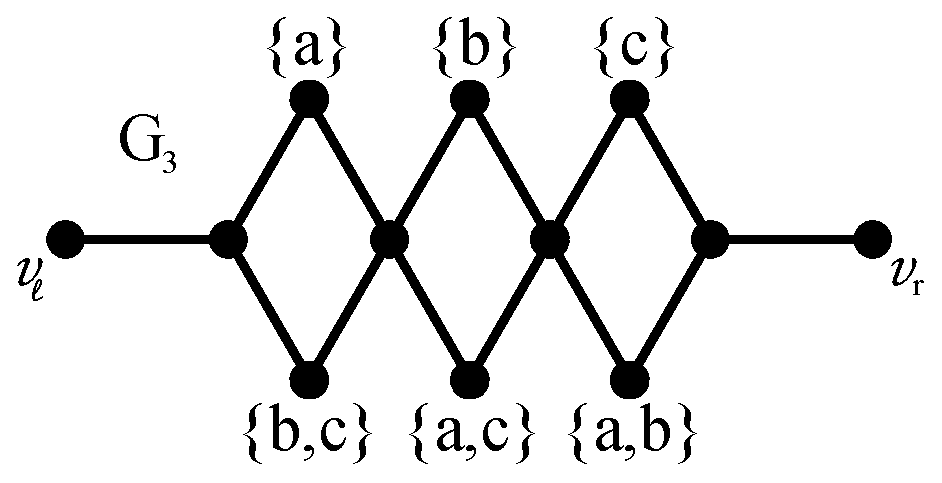
\includegraphics[scale=0.4]{figures/eps/tight-mapexample}
    \caption{An example of the $\mathsf{r}$ map for $G_3$. The set next to
    each top and bottom vertex $u$ is the set $s$ such that $\mathsf{r}(s)=u$.}
    \label{fig:mapexample}
  \end{figure}
  
  We now show that for each $s\in S$, $s=Q\cap\mathcal{T}_{\mathsf{r}(s)}$. This
  is easy to see as $\mathsf{r}(s)$ is internal to all paths in $s$, by
  definition of $\mathsf{r}(s)$ and of the paths in $Q$. On the other end, no
  path from $\mathsf{c}(s)$ goes through $\mathsf{r}(s)$ because it goes through
  the corresponding vertex of $\mathsf{r}(s)$ (top if $\mathsf{r}(s)$ is a
  bottom vertex, bottom otherwise). It is also straightforward to see that,
  if we let $v_Q$ be any arbitrary middle vertex different from $v_\ell$
  or $v_\mathrm{r}$, we have $Q=Q\cap\mathcal{T}_{v_Q}$, given that all paths in
  $Q$ go through all the middle vertices. Also, given that $v_\ell$ is not
  internal to any path, we have $\emptyset=Q\cap\mathcal{T}_{v_\ell}$. Then all
  subsets of $Q$ can be expressed as the intersection between $Q$ and a range
  from $\range_{G_d}$, which means that $Q$ can be shattered and therefore
  $\VC(\range_{G_d})\ge d$.

  From Lemma~\ref{lem:vcdimuppbound} we know that $\VC(\range_{G_d})\le d$, so
  it must be $\VC(\range_{G_d})=d$.
%\end{IEEEproof} 
\end{proof}
\else
Due to space constraints, we defer the proof to the extended online version of
the paper~\citep{RiondatoK13}.
\fi

The upper bound presented in Lemma~\ref{lem:vcdimuppboundunique}  for the case
of unique shortest paths is also strict in the same sense.
\ifproof
\else
The proof can be found in the extended online version of the
paper~\citep{RiondatoK13}.
\fi

\begin{lemma}\label{lem:vcdimlowboundunique}
  There is a graph $G=(V,E)$ with $|\mathcal{S}_{uv}|\le1$ for all
  pairs $(u,v)\in V\times V$ such that the range set $\range_G$ associated to the
  shortest paths in $G$ has VC-Dimension exactly $3$.
\end{lemma}

\ifproof
\begin{figure}[ht]
  \centering
  \begin{tikzpicture}
    \GraphInit[vstyle=Classic]
    \tikzset{VertexStyle/.append style = { minimum size = 2 pt }}
    \Vertex[Lpos=135]{a}
    \EA[Lpos=135](a){b}
    \EA[Lpos=135](b){c}
    \NO[Lpos=135](c){d}
    \EA[Lpos=135](c){e}
    \NO[Lpos=135](e){f}
    \NO[Lpos=135](f){g}
    \NOEA[Lpos=45](f){m}
    \NO[Lpos=135](g){h}
    \EA[Lpos=45](e){i}
    \NO[Lpos=45](i){j}
    \EA[Lpos=45](i){k}
    \EA[Lpos=45](k){l}
    \Edge(a)(b)
    \Edge(b)(c)
    \Edge(c)(d)
    \Edge(c)(e)
    \Edge(e)(f)
    \Edge(f)(g)
    \Edge(f)(m)
    \Edge(g)(h)
    \Edge(e)(i)
    \Edge(i)(j)
    \Edge(i)(k)
    \Edge(k)(l)
  \end{tikzpicture}
  %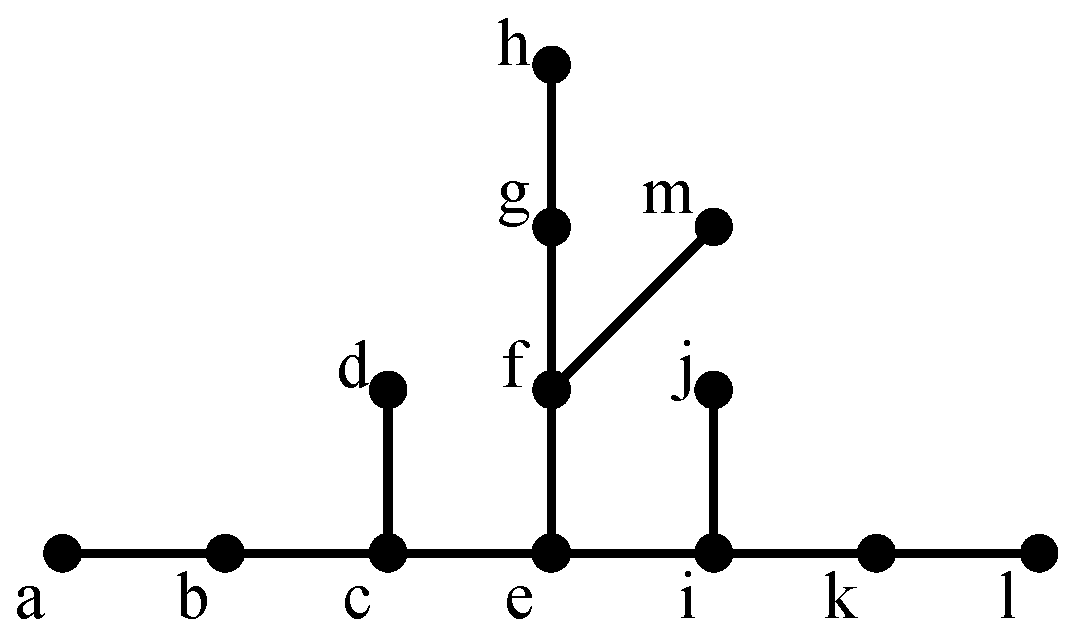
\includegraphics[scale=0.35]{figures/eps/uniqueshortestpathtight}
  \caption{Graph $G$ with $\VC(\range_G)= 3$.}
  \label{fig:uniquetight}
\end{figure}

\begin{proof}
%\begin{IEEEproof}
  Consider the graph $G$ in Fig.~\ref{fig:uniquetight}.
  Let $p_1=(a,b,c,e,i,j)$, $p_2=(m,f,e,i,k,l)$, $p_3=(d,c,e,f,g,h)$ be three
  paths. We now show that $Q=\{p_1,p_2,p_3\}$ can be shattered by $\range_G$, which
  implies $\VC(\range_G)\ge 3$. We have $\emptyset=Q\cap\mathcal{T}_a$,
  $\{p_1\}=Q\cap\mathcal{T}_b$, $\{p_2\}=Q\cap\mathcal{T}_k$,
  $\{p_3\}=Q\cap\mathcal{T}_g$, $\{p_1,p_2\}=Q\cap\mathcal{T}_i$,
  $\{p_1,p_3\}=Q\cap\mathcal{T}_c$, $\{p_2,p_3\}=Q\cap\mathcal{T}_f$,
  $\{p_1,p_2,p_3\}=Q\cap\mathcal{T}_e$,  
  Hence all subsets of $Q$ can be expressed as the intersection between $Q$ and
  some range in $\range_G$ which means that $Q$ can be shattered and
  $\VC(\range_G)\ge 3$. Lemma~\ref{lem:vcdimuppboundunique} gives us an upper
  bound $\VC(\range_G)\le3$, so we can conclude that $\VC(\range_G)=3$.
%\end{IEEEproof}
\end{proof}

Although the example in Fig.~\ref{fig:uniquetight} is a tree, this is not a
requirement for either Lemma~\ref{lem:vcdimuppboundunique} or
Lemma~\ref{lem:vcdimlowboundunique}: in a weighted graph with cycles (i.e., not
a tree) the weights may be such that there is a unique shortest path between any
pair of connected vertices.
\fi


\section{Algorithm}\label{sec:algo}
In this section we present our algorithm to compute a set of approximations for the
betweenness centrality of all vertices in a graph through sampling, with
probabilistic guarantees on the quality of the approximations.

The intuition behind the algorithm is the following. Given a graph $G=(V,E)$
with vertex-diameter $\Delta_g$ and two parameters $\varepsilon,\delta\in(0,1)$ we first compute a sample
size $k$ using~\eqref{eq:vceapprox} with
$d=\lfloor\log_2\Delta_G\rfloor+1$:
\begin{equation}\label{eq:samplesize}
k=\frac{c}{\varepsilon^2}\left(\lfloor\log_2\Delta_G\rfloor+1+\ln\frac{1}{\delta}\right)\enspace.
\end{equation}
The sample size is sufficient to ensure
to achieve the desired accuracy (expressed through $\varepsilon$) with the
desired confidence (expressed through $1-\delta$). Then the algorithm builds a
sample $S$ of $k$ shortest path from $\mathbb{S}_G$ by sampling them according to
the probability distribution $\prob_G$ defined on $\mathbb{S}_G$ as follows:
given a shortest path $p_{uv}\in\mathbb{S}_G$ between a pair of vertices
$(u,v)\in V\times V$, 
\[
\prob_G(p_{uv})=\frac{1}{\binom{n}{2}|\mathcal{S}_{uv}|}\enspace.%=\frac{2}{n(n-1)|\mathcal{S}_{uv}|}\enspace.
\]
Sampling according to $\prob_G$ can be achieved by first picking a pair of distinct vertices $(u,v)$
uniformly at random, computing the set $\mathcal{S}_{uv}$ of all the shortest
paths between $u$ and $v$, and selecting one of these shortest paths uniformly
at random. The estimation $\tilde\betw(v)$ of the betweenness centrality of each
vertex $v\in V$ is obtained by computing the fraction of shortest paths in $S$
that $v$ belongs to and de-normalizing it: 
\[
\tilde\betw(v) = \binom{n}{2}\frac{1}{k}\sum_{p\in S}
\mathds{1}_{p}(v) = \binom{n}{2}\frac{1}{k}\sum_{p\in S}
\mathds{1}_{\mathcal{T}_v}(p)\enspace.
\]
Algorithm \ref{alg:algorithm} presents the pseudocode.
\begin{algorithm}[ht]
  \SetKwInOut{Input}{Input}
  \SetKwInOut{Output}{Output}
  \SetKwFunction{VertexDiameter}{getVertexDiameter}
  \SetKwFunction{SamplePair}{sampleVertexPair}
  \SetKwFunction{SampleUniform}{sampleUniformPath}
  \SetKwFunction{PairShortestPaths}{computeAllShortestPaths}
   \DontPrintSemicolon
  %\dontprintsemicolon
  \Input{a graph $G=(V,E)$ with $|V|=n$, real values $\varepsilon,\delta\in(0,1)$}
  \Output{A set of approximations }
  $\Delta_G\leftarrow$\VertexDiameter{G}\label{alg:diamcomp}\; 
  $k\leftarrow (c/\varepsilon^2)(\lfloor\log_2\Delta_G\rfloor+\ln(1/\delta))$\;
  $S\leftarrow\emptyset$\;
  \For{$i\leftarrow 1$ to $k$} {
  $(u,v)\leftarrow$\SamplePair{$G$}\;
  $\mathcal{S}_{uv}\leftarrow$\PairShortestPaths{$(u,v)$}\;
  $s\leftarrow$\SampleUniform{$\mathcal{S}_{uv}$}\;
  $S\leftarrow S\cup\{s\}$\;
  }
  \For{$v\in V$} {
  $\tilde\betw(v)\leftarrow\binom{n}{2}\sum_{p\in S}\mathds{1}_{p}(v)$\;
  }
  \Return{$\{\tilde\betw(v), v\in V\}$}
  \caption{Computes approximations $\tilde\betw(v)$ of the betweenness
  centrality $\betw(v)$ for all vertices $v\in V$.}
  \label{alg:algorithm}
\end{algorithm}

The algorithm we describes offers probabilistic guarantees on the quality of all
approximations of the betweenness centrality.
\begin{lemma}\label{lem:correctness}
  With probability at least $1-\delta$, all the approximations computed by the
  algorithm are within $\varepsilon\binom{n}{2}$ from their real value:
  %The algorithm computes a set of approximations $\tilde\betw(v)$ for each $v\in
  %V$ such that
  \[
  \Pr\left(\exists v\in V \mbox{ s.t. }
  |\betw(v)-\tilde\betw(v)|>\varepsilon\binom{n}{2}\right)<\delta\enspace .
  \]
\end{lemma}

\begin{proof}
  Consider the range set $\range_G$ and the probability distribution $\prob_G$.
  For $k$ as in~\eqref{eq:samplesize}, the sample $S$ is a
  $\varepsilon$-approximation to $(\range_G,\prob_G)$ with probability at least
  $1-\delta$. Suppose that this is indeed the case, then from
  Def.~\ref{def:eapprox} and the definition of $\range_G$ we have that
  \[
  \left|\prob_G(\mathcal{T}_v) - \frac{1}{k}\sum_{p\in
  S}\mathds{1}_{\mathcal{T}_v}(p)\right|=\left|\prob_G(\mathcal{T}_v) -
  \frac{1}{\binom{n}{2}}\tilde\betw(v)\right|\le\varepsilon, \forall v\in
  V\enspace.
  \]
  From the definition of $\prob_G$ we have
  \[
  \prob_G(\mathcal{T}_v)=\frac{1}{\binom{n}{2}}\sum_{p_{uw}\in\mathcal{T}_v}\frac{1}{|\mathcal{S}_{uw}|}=\frac{1}{\binom{n}{2}}\betw(v),
  \]
  which concludes the proof.
\end{proof}

\subsection{Approximating the diameter}\label{sec:diam}
The algorithm presented in the previous section requires the knowledge (or the
computation) of the vertex-diameter $\Delta_G$) of the graph $G$ (line
\ref{alg:diamcomp} of Alg.~\ref{alg:algorithm}). Computing $\Delta_G$ exactly
can be done by finding the shortest paths between all pair of vertices in $V$
and computing the maximum size. This can be done in time \XXX. Such an exact
computation would defeat our purposes, because once we have all the shortest
paths, we can compute the betweenness of all the nodes exactly. Given that
Thm.~\ref{thm:eapprox} only requires an upper bound to the VC-dimension of the
range set, an upper bound to the vertex-diameter would be sufficient for our
purposes, provided its computation is fast and it does not result in a much
larger sample size than if we used the exact value for $\Delta_G$. There are
known algorithms the diameter of a graph \XXX references, discussion \MR
For our case, a $2$-approximation to $\Delta_G$ can be computed in time \XXX by selecting a
vertex $v\in V$ uniformly at random, computing the shortest path from $v$ to all
other vertices in $V$, and taking $\tilde\Delta_G$ to be the sum of the sizes of
the two longest shortest paths from $u$ to two distinct other nodes. 

\begin{lemma}
  $\tilde\Delta_G\le 2\Delta_G$.
\end{lemma}
\begin{proof}
  \XXX TBD but seems easy.
\end{proof}

The impact of using $\tilde\Delta_G$ when computing the sample size $k$ is that
the sample will contain at most $c/\varepsilon^2$ more paths than if we used the
exact value $\Delta_G$. 

\subsection{Discussion}
\XXX TBD: running time, worst case, comparison with best previous work.


\section{Experimental evaluation}\label{sec:exper}
We conducted and extensive experimental evaluation of our algorithm and
compared its performances with those of other existing algorithm, both
exact~\citep{Brandes01} and approximate~\citep{BrandesP08,JakobKLPT05}.

\paragraph{Goals} TBD

\paragraph{Implementation and environment}
We implemented our algorithm and the one presented
in~\citep{BrandesP08,JakobKLPT05} in C, by extending the implementation of the
exact algorithm~\citep{Brandes01} contained in igraph~\citep{igraph}. We
exposed our implementations through Python 3.3.1, which was used for running the
simulations. We run the experiments on a quad-core AMD Phenom\texttrademark II
X4 955 Processor with 16GB of RAM, running GNU/Linux 3.2.0.

\paragraph{Datasets} We used a number of datasets from the Stanford Large
Network Dataset
Collection\footnote{\url{http://snap.stanford.edu/data/index.html}}. These are
all real world networks including online social networks, communication (email)
networks, scientific citation and academic collaboration networks, road
networks, Amazon frequent co-purchased product networks, and more. We refer the
reader to the SLNDC website for details about each dataset.

\subsection{Runtime evaluation}\label{sec:runtime}
TBD

\subsection{Accuracy evaluation}\label{sec:accuracy}
TBD

\section{Conclusions}\label{sec:concl}
In this work we presented two random-sampling-based algorithms for accurately and
efficiently estimate the betweenness centrality of the (top-$K$) vertices in a
graph, with high probability.
%For very large graphs, exact computation of the
%betweenness centrality is impossible, so one has to resort to an approximation.
Our algorithms take a different approach than previous ones achieving the same
guarantees~\citep{BrandesP07,GeisbergerSS08,JacobKLPT05} as it is based on a
completely novel application of results from VC-dimension theory. These results
allow us to show that the number of samples needed to approximate the
betweenness with the desired accuracy and confidence is much smaller than that
suggested by previous works. Moreover, our algorithm performs much less work
per sample than other algorithms. We tested our algorithm on many real graphs
and showed that it is many times faster than other proposed methods. In future
work we would like to explore the possibility of extending our methods to
generalizations of betweenness centrality~\citep{DolevEP10} and to other centrality
measures. On the more theoretical side, we believe that the bound presented in
Lemma~\ref{lem:vcdimuppbound} is strict in the sense that there are graphs $G$
whose $\range_G$ has VC-dimension exactly $\lfloor\log_2\Delta_G\rfloor+1$, and
we have preliminary results in this sense that need formalization. 



\bibliographystyle{abbrvnat}
\bibliography{vcmine,centrality}


\end{document}

